\documentclass[11pt,english]{article}

\usepackage{siunitx}
\sisetup{range-phrase={ -- }}
\sisetup{range-units=single}
\usepackage{amsmath}
\newcommand\numberthis{\addtocounter{equation}{1}\tag{\theequation}}
\usepackage{amssymb}

\usepackage{mathspec}
\setallmonofonts[
  AutoFakeSlant,
  BoldItalicFeatures={FakeSlant},
  ]{Inconsolata}

\usepackage{polyglossia}
\setdefaultlanguage{english}
\usepackage{microtype}

\usepackage{float}
\usepackage{graphicx}
\usepackage[hypcap]{caption}

\usepackage{perpage}
\MakePerPage{footnote}

\usepackage{xcolor}
\definecolor{link}{HTML}{4078C0}
\usepackage[colorlinks=true, allcolors = link, linktoc = all]{hyperref}

\title{Lemta\texttrademark 10CC15C98T Clock/Countdown-Timer\\User notice}
\author{Nathan \textsc{Dwek} -- Ilias \textsc{Fassi Fihri}}


\begin{document}
\maketitle
\hypersetup{allcolors=black}
\tableofcontents
\hypersetup{allcolors=link}

\section{Device description}
The 10CC15C98T is a clock/countdown-timer with the following features:
\begin{itemize}
    \item \SI{24}{\hour} clock with second precision
    \item \SI{99}{\hour} countdown timer with second precision
    \item 6 digits digital display
    \item Programmable clock/countdown-timer using the intuitive numerical keypad
    \item Vintage mechanical display switch
    \item Countdown and input status leds
    \item Protection against faulty user inputs
\end{itemize}

Figure~\ref{fig:board} maps these features to the product you just acquired.
\begin{figure}[htbp]
    \centerline{%
    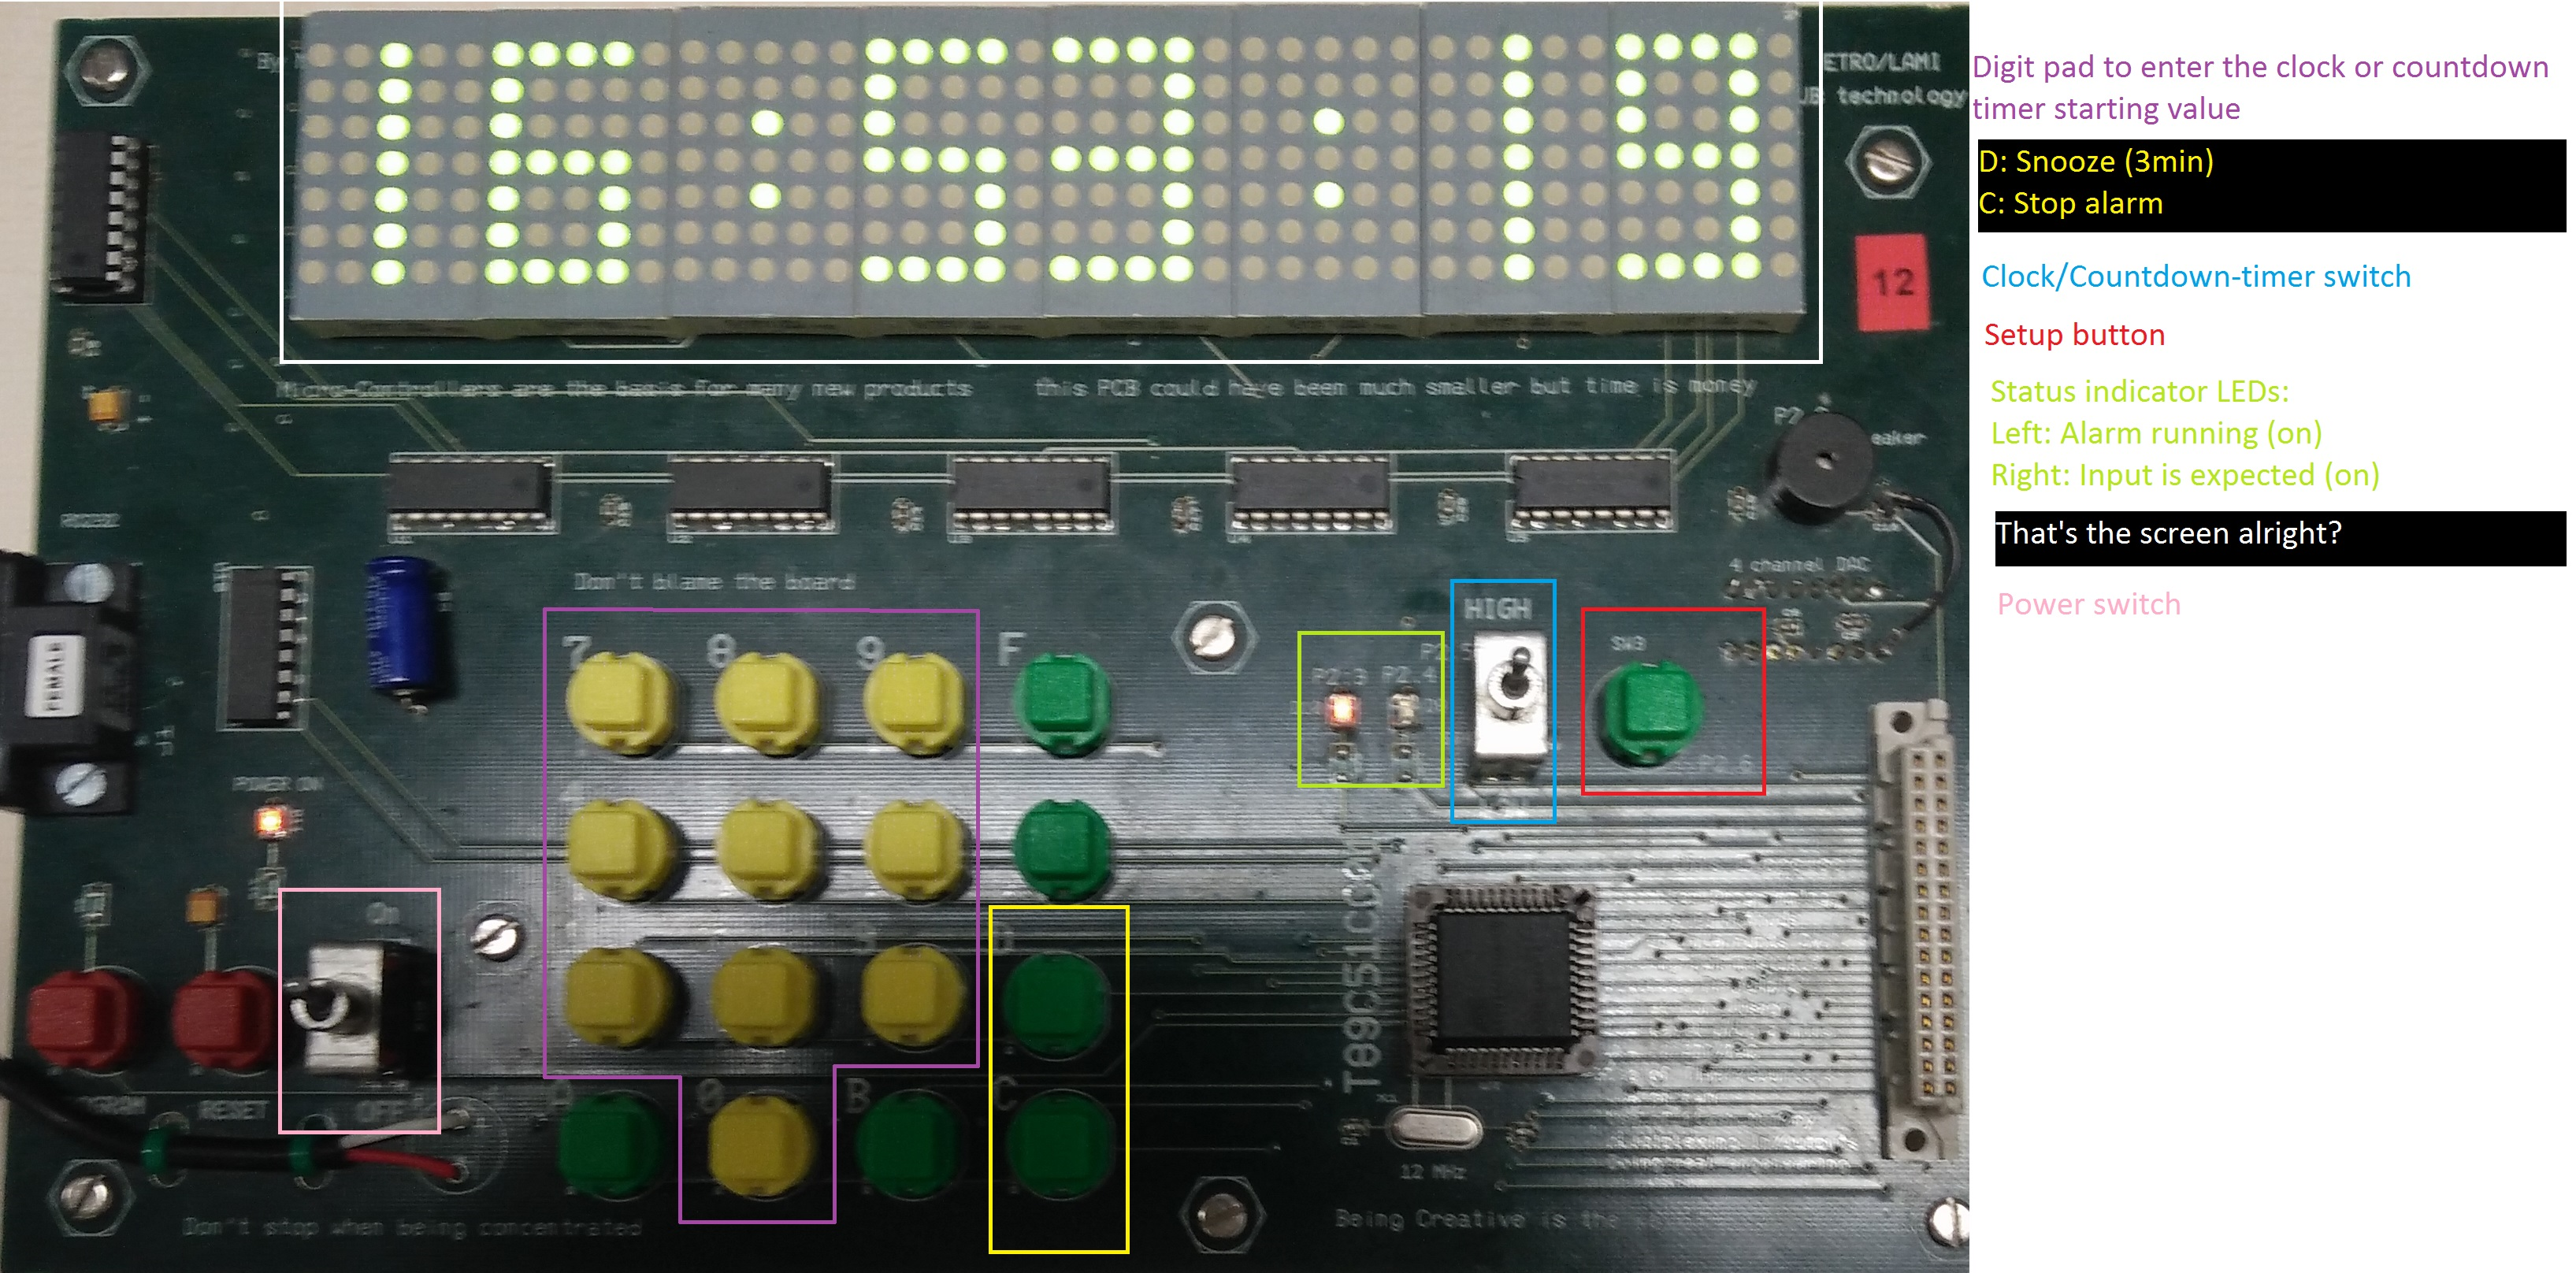
\includegraphics[width=1.1\textwidth]{board.jpg}}
    \caption{Visual description of the 10CC15C98T alarm-clock\label{fig:board}}
\end{figure}
We will now demonstrate how to use the device based on this device description.

\section{Device usage}
Before proceeding further, please make sure the device is turned on by turning on the power switch.
The display shows the clock when the clock/countdown switch is up, and the countdown timer when the switch is down. This switch also controls whether the user is setting up the clock or the countdown as we will see in the following subsections.

\subsection{Setting up the clock}
First, we invite you to set up the clock in order to maximize the device utility.
In order to do that, place the display switch on position up in order to show the clock.
The clock is running constantly and throughout the set up.
Then, press the setup button once.
The right status led (awaiting input) should light up as you release the button.
As long as this led is on, the device is waiting for an input and is not back to normal operation.

Next, enter the desired time using the numeric keypad, this should take six inputs, which are taken on the release.
When you are done, the right status led should turn off and the clock should continue running from the time you set up.

Every digit is protected against faulty user inputs. The clock uses 24h60m60s standard format

\subsection{Setting up the alarm}
To set up the alarm, follow the same procedure as to setup the clock, but with the display switch down.
Note, however, a few differences:
\begin{itemize}
    \item The countdown-timer stops when you press the setup button and doesn't restart until you released the sixth digit.
    \item This is additionnally indicated by the left status led which, regardless of the screen status, is on when the alarm is running, and off otherwise.
    \item The countdown timer is protected against user inputs, but allows times up to 99h59m59s.
\end{itemize}

When the countdown timer attains zero, the buzzer start ringing with a sweet melody. Beyond early morning suicide, the user can choose between three other possibilities:
\begin{itemize}
    \item Stop the alarm using button C.
    \item Snooze using button D. A 3 minutes countdown is automatically restarted.
    \item Re-enter any other new duration using the setup button and the numeric keypad as previously explained.
\end{itemize}

\section{Day to day operation and for experienced users}
On the day to day, use the display switch to consult the clock or the alarm whenever needed.
The display switch interrupts any current setup operation which should then be restarted from the beginning.
This is to ensure the user cannot modify values not currently displaying.

Experienced users will notice that it is thus possible to stop the timer at any time by pressing the setup button and then switching the display switch. It is however impossible to later restart the timer without setting it up entirely again.

Further modifications are possible using a micro-USB adapter (sold separately) and voodoo-ylbmessa incantations.
To that end, the source code and hex file of this device as well as a block diagram and a description of the memory organisation are provided with this notice.
\end{document}
